\section*{Exercise 1}
In this assignment, we implement the k-means algorithm for clustering the input data points.
Clustering is considered as a unsupervised machine learning problem, that means there no labels in the data that we need to predict as classification, but it helps us getting some insights about the input data.

We developed four methods for initializing the first K cluster centroids (where K is an input)
The first one is just choosing the first K data points to be the centroids, the second method is randomized selections of the initial centroids. the third method is k-means++
and the fourth method is using Gonzales’ algorithm.

For each method, we run k-means for different values of k {3,4,5} and in randomized methods, we run that 5 times. we visualise the results to get more understanding and learning experience as shown below.


\begin{figure}[!htb]
\centering
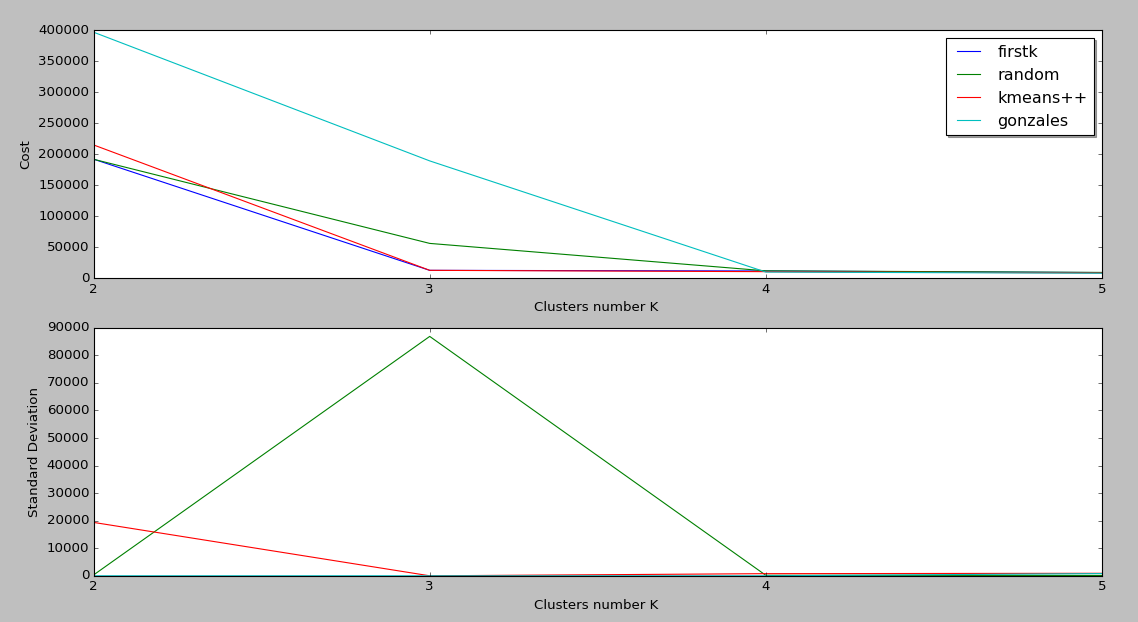
\includegraphics[width=0.9\textwidth]{shots/std_mean.png}
\caption{The average costs(top) and average Standard deviations(bottom) of several runs of k-means for different clusters numbers and using different methods of initialization.}
\label{std_mean}
\end{figure}

The top digram of figure \ref{std_mean} shows the average cost of 5 runs of each method of initialization for k-means for different number of clusters, we can see that Gonzales method has the worst average cost across all the methods for 2 and 3 clusters. Starting of 4, all the method has similar costs on average. The reason for this is the distribution of the data points in the file C2 where we can find an outlier point that's very far of most of the points. this point is always chosen by Gonzales' algorithm as a center of one of the clusters.

The bottom figure shows standard deviation of the costs across all the 5 runs. and we can see the random initialization can have higher standard deviation which means that one or more of the runs can be highly deviated from average of the runs.


\begin{figure}[!htb]
\centering
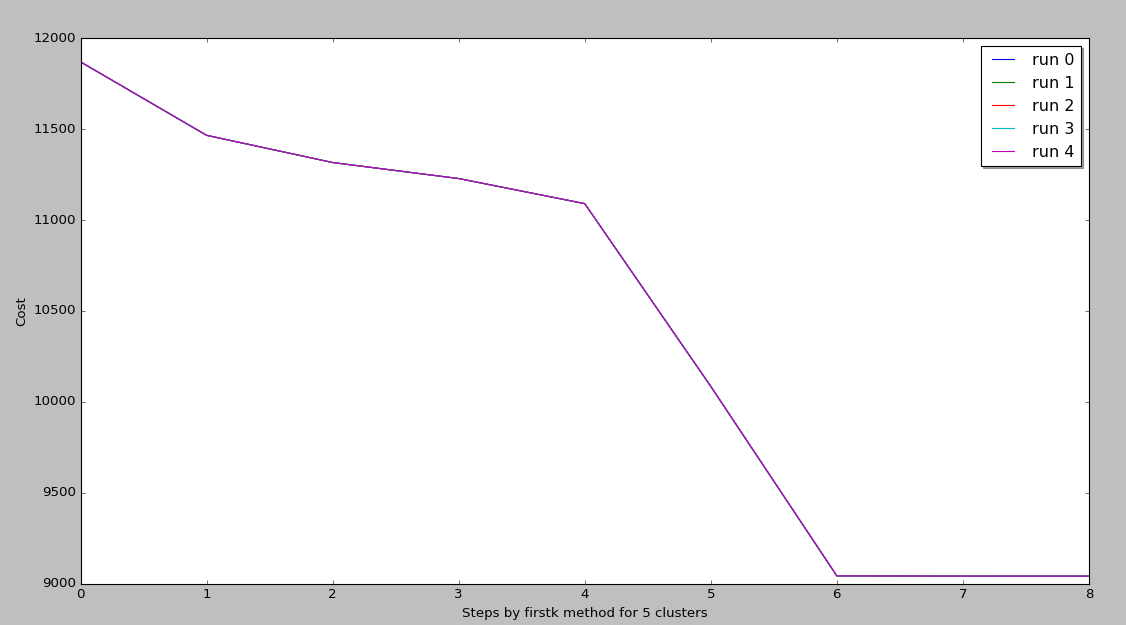
\includegraphics[width=0.9\textwidth]{shots/firstk5clusters.png}
\caption{Convergent rate of k-means using the first 5 points as initial centroids. }
\label{firstk5clusters}
\end{figure}


Figure \ref{firstk5clusters} shows the convergence rate of k-means algorithm using the first 5 points as the initial centroids, we can see that of course it will be same if run this several times as no randomization exists.


\begin{figure}[!htb]
\centering
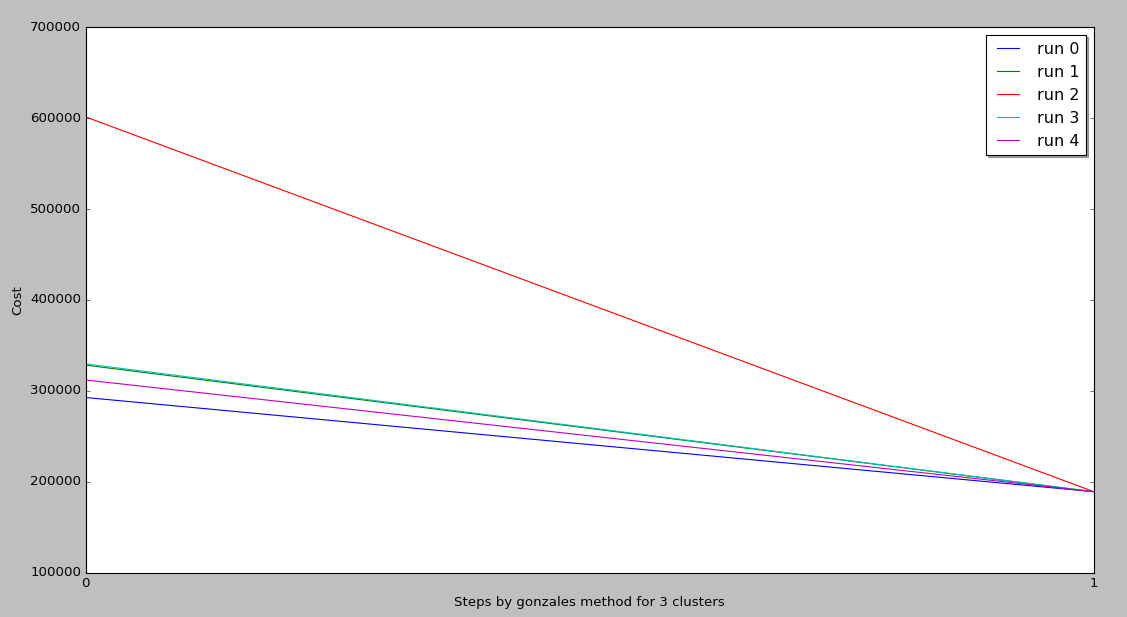
\includegraphics[width=0.9\textwidth]{shots/gonzales3clusters.png}
\caption{Convergence rate of k-means using initialization of Gonzales' algorithm and 3 clusters for 5 different runs }
\label{gonzales3clusters}
\end{figure}

\begin{figure}[!htb]
\centering
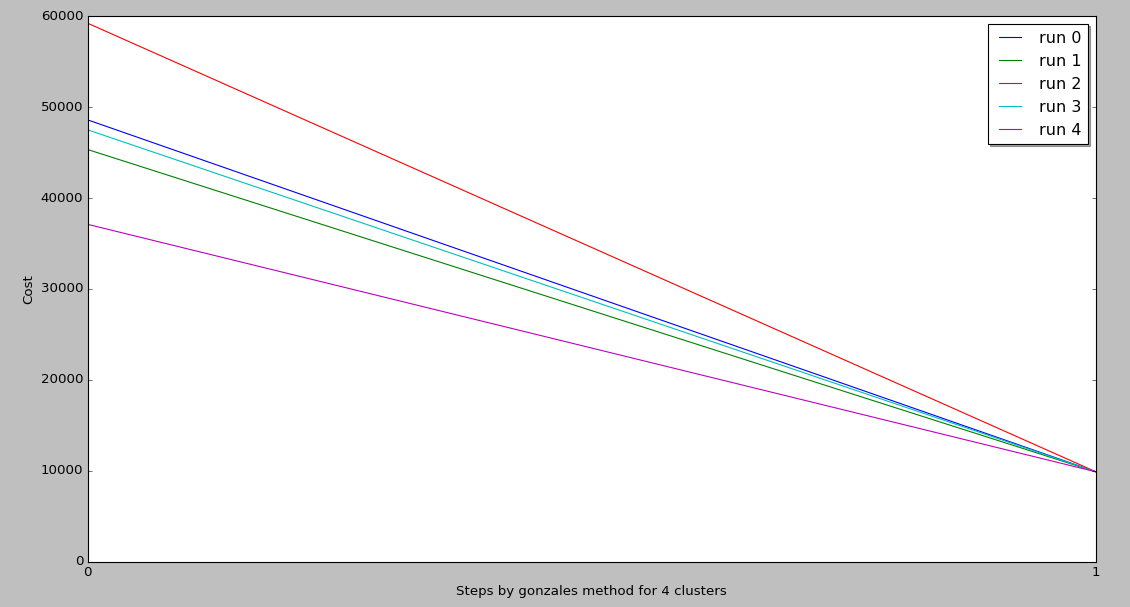
\includegraphics[width=0.9\textwidth]{shots/gonzales4clusters.png}
\caption{Convergence rate of k-means using initialization of Gonzales' algorithm and 4 clusters for 5 different runs  }
\label{gonzales4clusters}
\end{figure}

\begin{figure}[!htb]
\centering
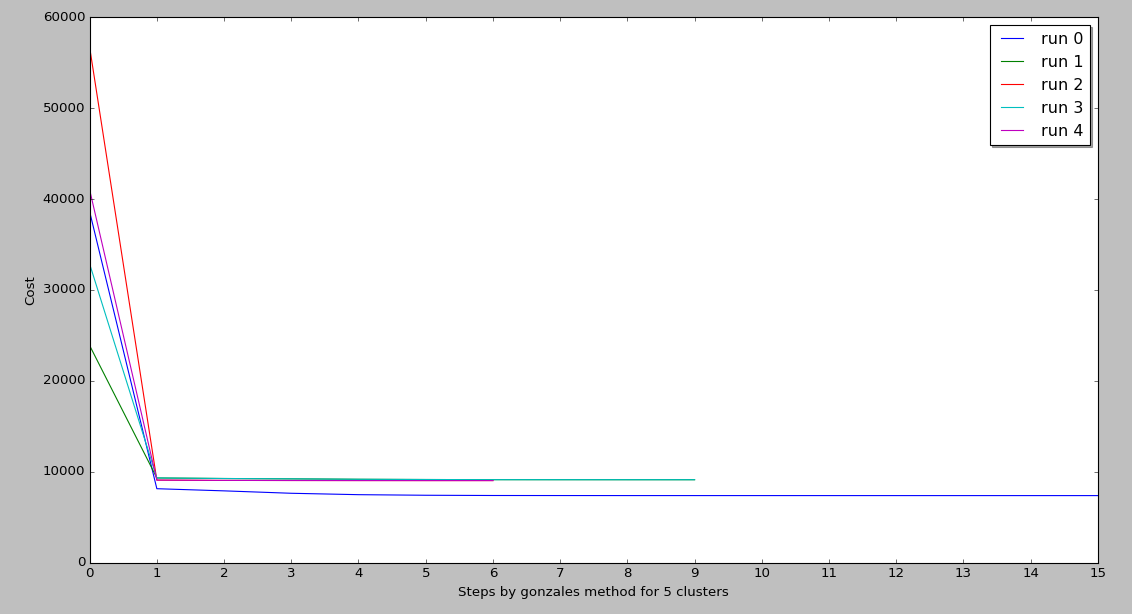
\includegraphics[width=0.9\textwidth]{shots/gonzales5clusters.png}
\caption{ Convergence rate of k-means using initialization of Gonzales' algorithm and 5 clusters for 5 different runs }
\label{gonzales5clusters}
\end{figure}

Figure \ref{gonzales3clusters} and \ref{gonzales4clusters} shows the convergent rate of k-means algorithm of 3 clusters using Gonzales's algorithm centers as the initial centroids, we can see it converged in just one step.

But for 5 clusters Gonzales' algorithm convergent rate was diverse between 1 and 15 steps as in figure \ref{gonzales5clusters}.

\begin{figure}[!htb]
\centering
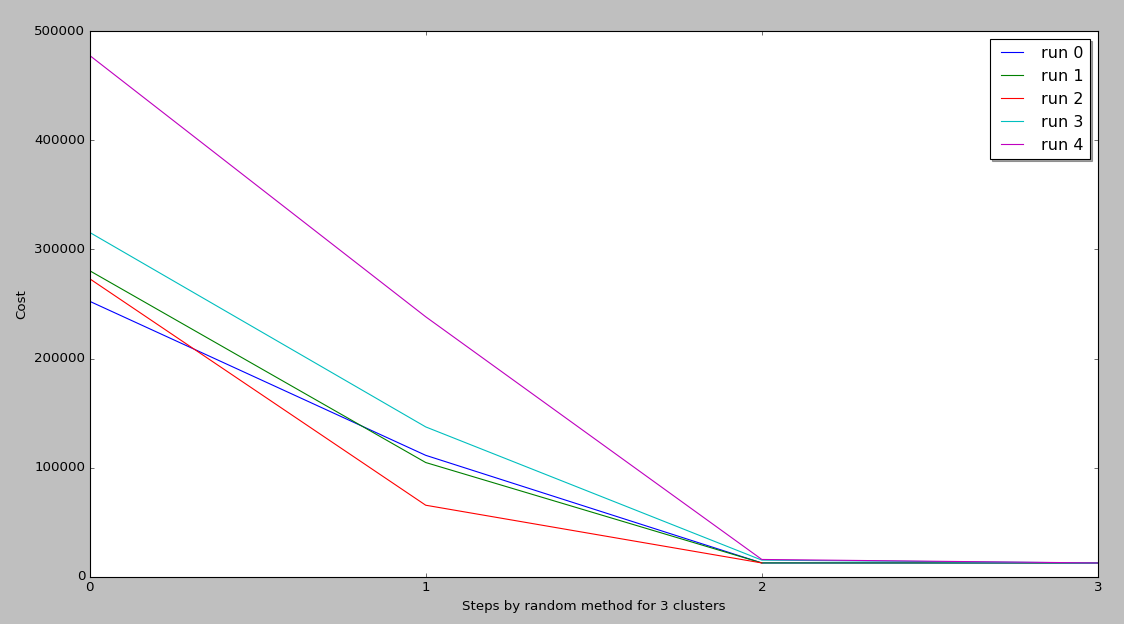
\includegraphics[width=0.9\textwidth]{shots/random3clusters.png}
\caption{ Convergence rate of k-means using random initialization and 3 clusters for 5 different runs }
\label{random3clusters}
\end{figure}



\begin{figure}[!htb]
\centering
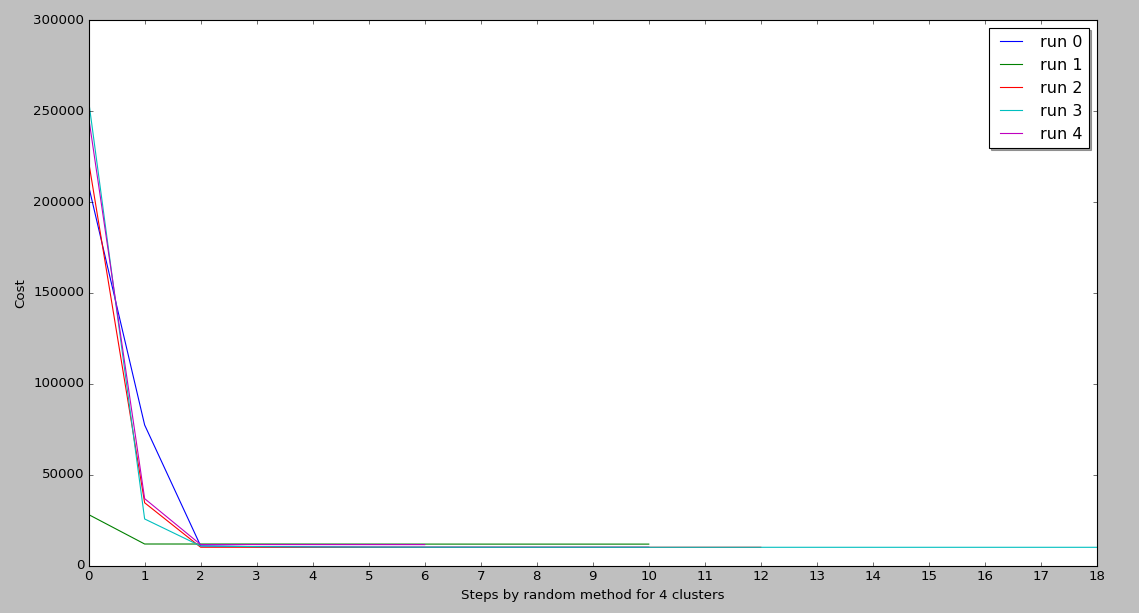
\includegraphics[width=0.9\textwidth]{shots/random4clusters.png}
\caption{ Convergence rate of k-means using random initialization and 4 clusters for 5 different runs }
\label{random4clusters}
\end{figure}



\begin{figure}[!htb]
\centering
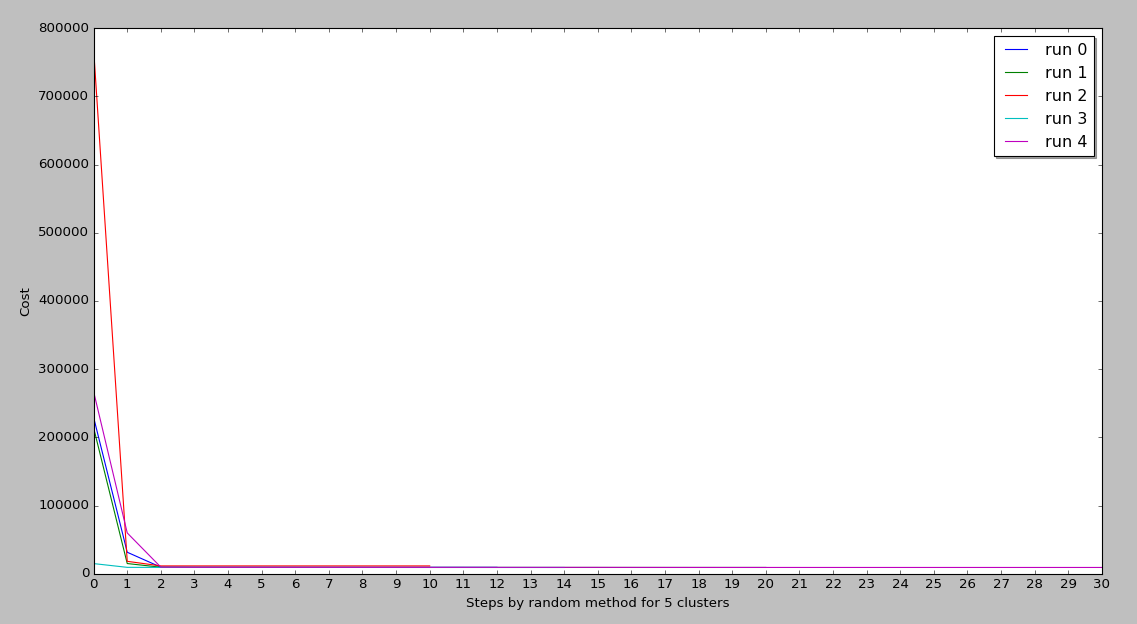
\includegraphics[width=0.9\textwidth]{shots/random5clusters.png}
\caption{ Convergence rate of k-means using random initialization and 5 clusters for 5 different runs  }
\label{random5clusters}
\end{figure}


Doing the same for the random method we can see in figures \ref{random3clusters} , \ref{random4clusters} and \ref{random5clusters} that for 3,4 and 5 clusters we can see different rates of convergence in each of the 5 runs per cluster number, that shows k-means algorithm is dependent on the initial centroids.

\begin{figure}[!htb]
\centering
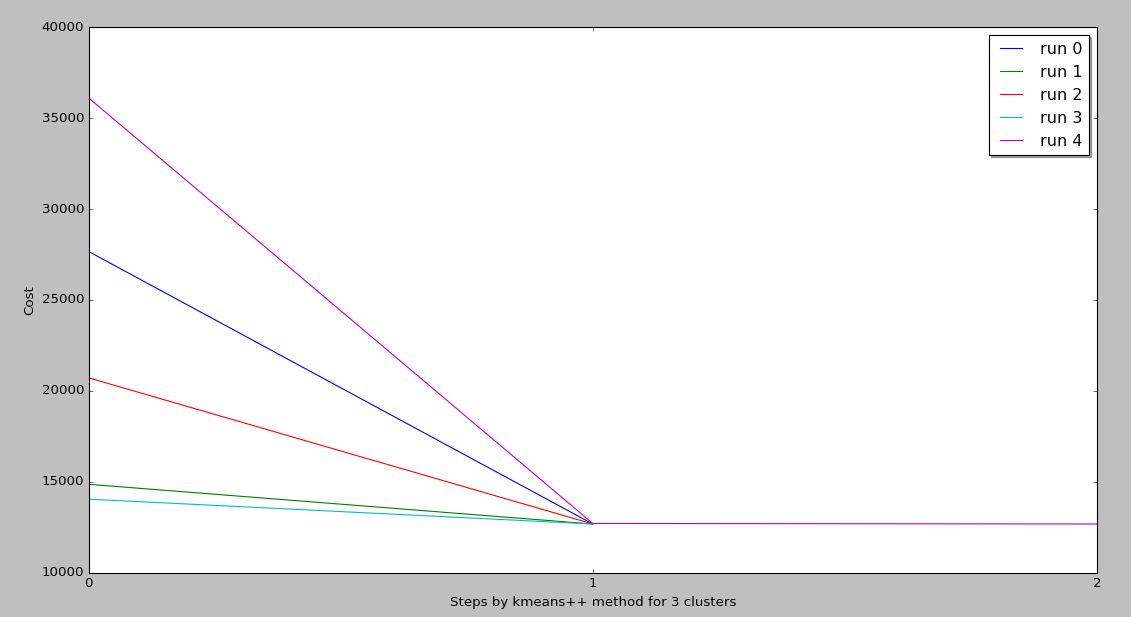
\includegraphics[width=0.9\textwidth]{shots/kmeans++3clusters.png}
\caption{ Convergence rate of k-means using kmeans++ initialization and 3 clusters for 5 different runs   }
\label{kmeans++3clusters}
\end{figure}



\begin{figure}[!htb]
\centering
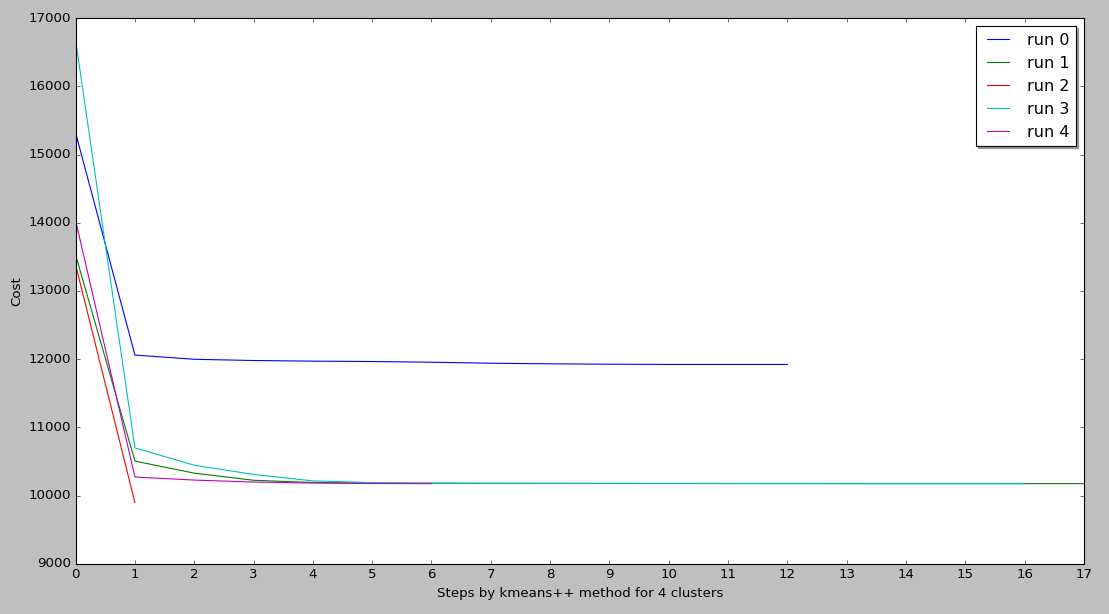
\includegraphics[width=0.9\textwidth]{shots/kmeans++4clusters.png}
\caption{Convergence rate of k-means using kmeans++ initialization and 4 clusters for 5 different runs  }
\label{kmeans++4clusters}
\end{figure}


\begin{figure}[!htb]
\centering
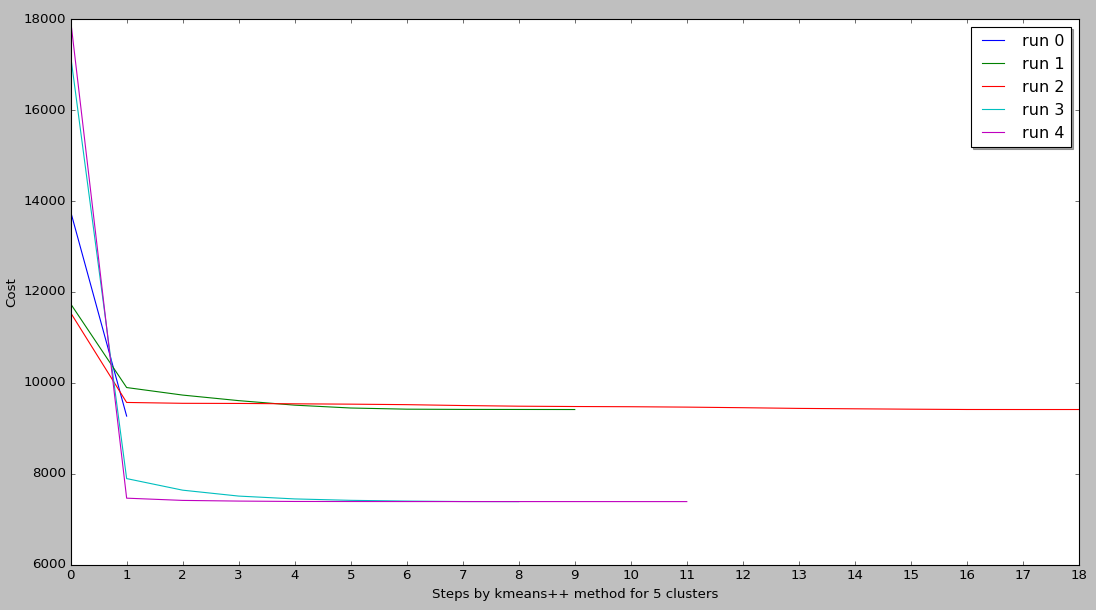
\includegraphics[width=0.9\textwidth]{shots/kmeans++5clusters.png}
\caption{ Convergence rate of k-means using kmeans++ initialization and 5 clusters for 5 different runs }
\label{kmeans++5clusters}
\end{figure}
  

For kmeans++ we ran the algorithm 5 times for each different clusters number to visualize the convergence rate as in figures \ref{kmeans++3clusters} , \ref{kmeans++4clusters} and \ref{kmeans++5clusters}. We can that the rates are also diverse across diffrent runs but on average k-means converge in less number of steps due to the intelligence of kmeans++ and choosing the initial centroids. 















